\section{Experimental Setup}
\label{subsec:supp-experiments-setup}

\textbf{Datasets:} We conduct experiments on \MNIST\footnote{\url{http://yann.lecun.com/exdb/mnist/}} \citep{LecunIEEE1998} and \Cifar\footnote{\url{https://www.cs.toronto.edu/~kriz/cifar.html}} \cite{Krizhevsky2009}. \MNIST consists of $60\text{k}$ training and $10\text{k}$ test images from $10$ classes. These are gray-scale and of size $28 \times 28$ pixels. \Cifar consists of $50\text{k}$ training and $10\text{k}$ test images of size $32\times 32\times 3$ (\ie, color images). \CifarT has images corresponding to $10$ classes, \CifarH contains images from $100$ classes.

\begin{table}[t]
	\centering
	\small
	\caption{\textbf{Weight Clipping with Weight Scaling.} For group normalization (GN) without the reparameterization in \secref{subsec:robustness-clipping}, using fixed scale/bias instead, our DNNs are scale-invariant. Scaling \Quant down to the weight range of \Clipping[$0.25$], however, does not improve robustness. Thus, the robustness benefit of \Clipping is \emph{not} due to reduced quantization range or smaller absolute errors.}
	\label{tab:supp-clipping-scaling}
	\vspace*{-0.25cm}
	\begin{tabular}{| l | c | c | c |}
		\hline
		\multicolumn{4}{| c |}{\bfseries \CifarT ($\mathbf{m = 8}$ bit): scaling w/o reparameterized GN}\\
		\hline
		Model & \multirow{2}{*}{\begin{tabular}{@{}c@{}}\TE\\in \%\end{tabular}} & \multicolumn{2}{c|}{\RTE in \%, $p$ in \%}\\
		\hline
		(see text) & & $p{=}0.1$ & $p{=}1$\\
		\hline
		\hline
		\Quant & 4.67 & 6.12 {\color{gray}\scriptsize ${\pm}$0.2} & 35.25 {\color{gray}\scriptsize ${\pm}$6.41}\\
		\Clipping[$0.25$] & 4.96 & 6.13 {\color{gray}\scriptsize ${\pm}$0.16} & 16.09 {\color{gray}\scriptsize ${\pm}$1.85}\\
		\hline
		\Quant $\rightarrow$ \Clipping[$0.25$] & 4.64 & 6.10 {\color{gray}\scriptsize ${\pm}$0.18} & 35.28 {\color{gray}\scriptsize ${\pm}$5.82}\\
		\hline
	\end{tabular}
	\vspace*{-0.1cm} 
\end{table}
\begin{figure*}[t]
	\centering
	\vspace*{-0.2cm}
	\begin{subfigure}{0.35\textwidth}
		\vspace*{0px}
		\centering
		\Quant
		
		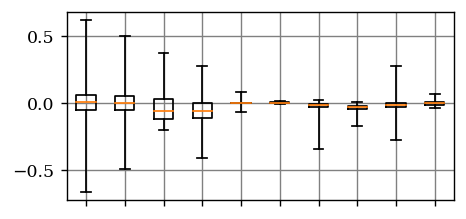
\includegraphics[width=1\textwidth]{c10_weights_q81auunrfp_nt.png}
	\end{subfigure}
	\begin{subfigure}{0.35\textwidth}
		\vspace*{0px}
		\centering
		\Random (w/o weight clipping)
		
		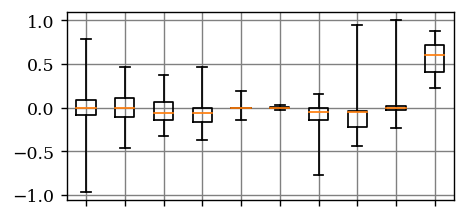
\includegraphics[width=1\textwidth]{c10_weights_q81auunrfp_sawt_bit_random_g001_pop1.png}
	\end{subfigure}
	\\
	\begin{subfigure}{0.35\textwidth}
		\vspace*{0px}
		\centering
		\Clipping[$0.1$]
			
		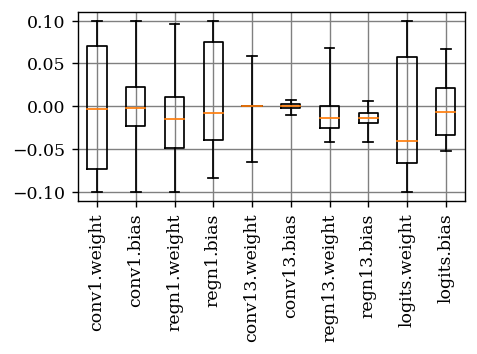
\includegraphics[width=1\textwidth]{c10_weights_q801auunrfp_nt.png}
	\end{subfigure}
	\begin{subfigure}{0.35\textwidth}
		\vspace*{0px}
		\centering
		\Clipping[$0.05$]
			
		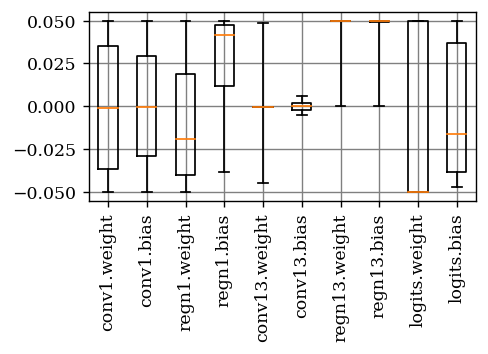
\includegraphics[width=1\textwidth]{c10_weights_q8005auunrfp_nt.png}
	\end{subfigure}
	\\
	\begin{subfigure}{0.16\textwidth}
		\vspace*{0px}
		\centering
		\Quant
		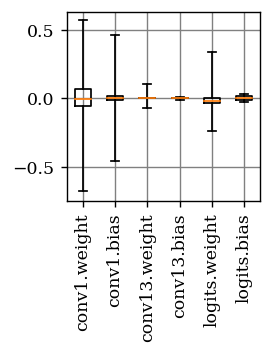
\includegraphics[width=1\textwidth]{c10_weights_q81auunrfp_nt_fixedgn.png}
	\end{subfigure}
	\begin{subfigure}{0.16\textwidth}
		\vspace*{0px}
		\centering
		\Clipping[$0.25$] $\uparrow$
			
		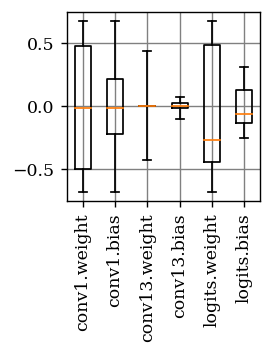
\includegraphics[width=1\textwidth]{c10_weights_q801auunrfp_nt__1p_fixedgn.png}
	\end{subfigure}
	\begin{subfigure}{0.35\textwidth}
		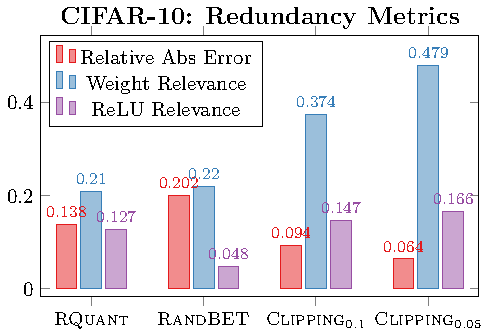
\includegraphics[width=1\textwidth]{c10_clipping}
	\end{subfigure}
	\vspace*{-6px}
	\caption{\textbf{Weight Clipping Increases Redundancy.} We show weight distributions of selected layers (top) for \Quant, \Random (without weight clipping) as well as \Clipping[$0.1$] and \Clipping[$0.05$]. We show weights and biases for the logit layer as well as the first and last (13th) convolutional layer. Scale/Bias parameters of GN are also included. Below (left), this is shown for the scaling experiment from \tabref{tab:supp-clipping-scaling} (GN parameters are fixed). Note that \Random only affects the logit layer, while \Clipping increases the used (relative) weight range significantly. On the bottom (right), we plot various measures of redundancy, see the text for discussion and details. The relative absolute error is computed considering random bit errors with probability $p = 1\%$.}
	\label{fig:supp-clipping}
	\vspace*{-0.1cm}
\end{figure*}

\textbf{Architecture:} The used SimpleNet architectures \cite{HasanpourARXIV2016} are summarized in \tabref{tab:supp-architectures}, including the total number of weights $W$. On \Cifar, this results in a total of roughly $W \approx 5.5\text{M}$ weights. Due to the lower resolution on \MNIST, channel width in each convolutional layer is halved, and one stage of convolutional layers including a pooling layer is skipped. This results in a total of roughly $W \approx 1\text{M}$ weights. In both cases, we replaced batch normalization (BN) \cite{IoffeICML2015} with group normalization (GN) \cite{WuECCV2018}. The GN layers are reparameterized as in \appref{sec:supp-clipping} to facilitate weight clipping. \tabref{tab:supp-architectures} also includes the expected number of bit errors given various rates $p$ for random bit errors. Regarding the number of weights $W$, SimpleNet compares favorably to, \eg, VGG \cite{SimonyanICLR2015}: VGG-16 has $14\text{M}$ weights on \Cifar. Additionally, we found SimpleNet to be easier to train without BN, which is desirable as BN reduces robustness to bit errors significantly, \cf \appref{subsec:supp-experiments-bn}. The ResNet-50 \cite{HeCVPR2016} used for experiments in \appref{subsec:supp-experiments-architectures} follows the official PyTorch \cite{PaszkeNIPSWORK2017} implementation. The Wide ResNet (WRN) \cite{ZagoruykoBMVC2016} used on \CifarH is adapted from\footnote{\url{https://github.com/meliketoy/wide-resnet.pytorch}}, but we use $12$ base channels, instead of $16$, reducing $W$ from roughly $36.5\text{Mio}$ to $20.5\text{Mio}$.

\begin{table*}[t]
	\centering
	\small
	\caption{\textbf{\Random Robustness with \emph{Symmetric} Quantization.} Average \RTE and standard deviation for \Clipping and \Random with $\wmax = 0.1$ and \textbf{s}ymmetric quantization, \ie, larger quantization range than {\color{red}a}symmetric quantization. Also \cf \tabref{tab:supp-clipping} and \tabref{tab:supp-summary-cifar10}. Robustness decreases slightly compared to asymmetric quantization, however, \Clipping and \Random are still effective in reducing \RTE against high bit error rates $p$.}
	\label{tab:supp-randbet-symmetric}
	\vspace*{-0.25cm}
	\begin{tabular}{|l | c | c | c | c | c | c | c |}
		\hline
		\multicolumn{8}{|c|}{\bfseries \CifarT ($\mathbf{m = 8}$ bit): \Random with symmetric quantization}\\
		\hline
		Model & \multirow{2}{*}{\begin{tabular}{c}\TE\\in \%\end{tabular}} & \multicolumn{6}{c|}{\RTE in \%, $p$ in \% p=0.01}\\
		\cline{3-8}
		&& $0.01$ & $0.05$ & $0.1$ & $0.5$ & $1$ & $1.5$\\
		\hline
		\hline
		\Normal & 4.36 & 4.82 {\color{gray}\scriptsize ${\pm}$0.07} & 5.51 {\color{gray}\scriptsize ${\pm}$0.19} & 6.37 {\color{gray}\scriptsize ${\pm}$0.32} & 24.76 {\color{gray}\scriptsize ${\pm}$4.71} & 72.65 {\color{gray}\scriptsize ${\pm}$6.35} & 87.40 {\color{gray}\scriptsize ${\pm}$2.47}\\
		\Quant & 4.39 & 4.77 {\color{gray}\scriptsize ${\pm}$0.08} & 5.43 {\color{gray}\scriptsize ${\pm}$0.21} & 6.10 {\color{gray}\scriptsize ${\pm}$0.32} & 17.11 {\color{gray}\scriptsize ${\pm}$3.07} & 55.35 {\color{gray}\scriptsize ${\pm}$9.4} & 82.84 {\color{gray}\scriptsize ${\pm}$4.52}\\
		\Clipping[$0.1$] & 4.86 & 5.07 {\color{gray}\scriptsize ${\pm}$0.04} & 5.34 {\color{gray}\scriptsize ${\pm}$0.06} & 5.59 {\color{gray}\scriptsize ${\pm}$0.1} & 7.12 {\color{gray}\scriptsize ${\pm}$0.3} & 9.44 {\color{gray}\scriptsize ${\pm}$0.7} & 13.14 {\color{gray}\scriptsize ${\pm}$1.79}\\
		\hline
		\Random[$0.1$] $p{=}0.01$ & 5.07 & 5.27 {\color{gray}\scriptsize ${\pm}$0.04} & 5.54 {\color{gray}\scriptsize ${\pm}$0.07} & 5.73 {\color{gray}\scriptsize ${\pm}$0.11} & 7.18 {\color{gray}\scriptsize ${\pm}$0.29} & 9.63 {\color{gray}\scriptsize ${\pm}$0.9} & 13.81 {\color{gray}\scriptsize ${\pm}$2.2}\\
		\Random[$0.1$] $p{=}0.1$ & 4.62 & 4.83 {\color{gray}\scriptsize ${\pm}$0.04} & 5.09 {\color{gray}\scriptsize ${\pm}$0.08} & 5.31 {\color{gray}\scriptsize ${\pm}$0.08} & 6.70 {\color{gray}\scriptsize ${\pm}$0.28} & 8.89 {\color{gray}\scriptsize ${\pm}$0.59} & 12.20 {\color{gray}\scriptsize ${\pm}$1.33}\\
		\Random[$0.1$] $p{=}1$ & 5.03 & 5.22 {\color{gray}\scriptsize ${\pm}$0.04} & 5.43 {\color{gray}\scriptsize ${\pm}$0.06} & 5.61 {\color{gray}\scriptsize ${\pm}$0.07} & 6.56 {\color{gray}\scriptsize ${\pm}$0.13} & 7.70 {\color{gray}\scriptsize ${\pm}$0.26} & 8.99 {\color{gray}\scriptsize ${\pm}$0.42}\\
		\Random[$0.1$] $p{=}1.5$ & 5.24 & 5.37 {\color{gray}\scriptsize ${\pm}$0.03} & 5.57 {\color{gray}\scriptsize ${\pm}$0.06} & 5.76 {\color{gray}\scriptsize ${\pm}$0.07} & 6.66 {\color{gray}\scriptsize ${\pm}$0.14} & 7.62 {\color{gray}\scriptsize ${\pm}$0.25} & 8.71 {\color{gray}\scriptsize ${\pm}$0.42}\\
		\Random[$0.1$] $p{=}2$ & 5.82 & 5.97 {\color{gray}\scriptsize ${\pm}$0.04} & 6.19 {\color{gray}\scriptsize ${\pm}$0.07} & 6.37 {\color{gray}\scriptsize ${\pm}$0.09} & 7.22 {\color{gray}\scriptsize ${\pm}$0.19} & 8.03 {\color{gray}\scriptsize ${\pm}$0.23} & 8.96 {\color{gray}\scriptsize ${\pm}$0.38}\\
		\hline
	\end{tabular}
	\vspace*{-0.1cm}
\end{table*}

\textbf{Training:} As outlined in \secref{sec:experiments}, we use stochastic gradient descent to minimize cross-entropy loss. We use an initial learning rate of $0.05$, multiplied by $0.1$ after $\nicefrac{2}{5}$, $\nicefrac{3}{5}$ and $\nicefrac{4}{5}$ of $100$/$250$ epochs on \MNIST/\Cifar. Our batch size is $128$ and momentum of $0.9$ is used together with weight decay of $5\cdot10^{-4}$. On \Cifar, we whiten the input images and use AutoAugment\footnote{\url{https://github.com/DeepVoltaire/AutoAugment}} \cite{CubukARXIV2018} with Cutout \cite{DevriesARXIV2017}. Cutout is applied with a window size of $16 \times 16$, and independent of AutoAugment, we apply random cropping with up to $4$ pixels. Created black spaces are filled using the mean image color (grayish). Initialization follows \cite{HeICCV2015}. The full training set is used for training, and we do \emph{not} rely on early stopping. For \Random, we use $\lambda = 1$ and start injecting bit errors when the loss is below 1.75 on \MNIST/\CifarT or 3.5 on \CifarH. \tabref{tab:supp-accuracy} highlights clean test error (\TE) obtained for various precision $m$ and compared to other architectures, \eg, ResNet-50, on \CifarT, which performs worse when using GN.

\textbf{Random Bit Errors:} We simulate $50$ different chips with enough memory arrays to accomodate all weights by drawing uniform samples $u^{(c)} \sim U(0, 1)^{W \times m}$ for each chip $c$ and all $m$ bits for a total of $W$ weights. Then, for chip $c$, bit $j$ in weight $w_i$ is flipped iff $u^{(c)}_{ij} \leq p$. This assumes a linear memory layout of all $W$ weights. The pattern, \ie, spatial distribution, of bit errors for chip $c$ is fixed by $u^{(c)}$, while across all $50$ chips, bit errors are uniformly distributed. We emphasize that we pre-determine $u^{(c)}$, $c = 1,\ldots,50$, once for all our experiments using fixed random seeds. Thus, our robustness results are entirely comparable across all models as well as bit error rates $p$. Also note that, as explained in \secref{sec:errors}, the bit errors for a fixed chip $c$ at probability $p' < p$ are a subset of those for bit error rate $p$. The expected number of bit errors for various rates $p$ is summarized in \tabref{tab:supp-architectures}.

\textbf{Implementation Details} are covered in \secref{sec:supp-implementation}.

\section{Experiments}
\label{sec:supp-experiments}

\subsection{Batch Normalization}
\label{subsec:supp-experiments-bn}

We deliberately replace batch normalization (BN) \cite{IoffeICML2015} by group normalization (GN) \cite{WuECCV2018} in our experiments. \tabref{tab:supp-bn} demonstrates that \RTE increases significantly when using BN compared to GN indicating that BN is more vulnerable to bit errors in DNN weights. For example, without clipping, \RTE increases from $11.28\%$ to staggering $52.52\%$ when replacing GN with BN. Note that, following \appref{sec:supp-clipping}, the BN/GN parameters (\ie, scale/bias) are reparameterized to account for weight clipping. The observations in \tabref{tab:supp-bn} can also be confirmed without quantization, \eg, considering random $L_\infty$ noise in the weights. We suspect that the running statistics accumulated during training do not account for the random bit errors at test time, even for \Random. This is confirmed in \tabref{tab:supp-bn} (bottom) showing that \RTE reduces significanlty when using the batch statistics at test time. Generally, BN improves accuracy, but might not be beneficial in terms of robustness, as also discussed for adversariale examples \cite{GallowayARXIV2019}. Using GN also motivates our use of SimpleNet instead of, \eg, ResNet-50, which generally performs worse with GN, \cf \tabref{tab:supp-accuracy}.

\subsection{Robust Quantization}
\label{subsec:supp-experiments-quantization}

\tabref{tab:supp-quantization} shows results complementary to the main paper, considering additional bit error rates $p$. Note that, for $m = 8$ bit, changes in the quantization has neglegible impact on clean \TE. Only the change from gloabl to per-layer quantization makes a difference. However, considering \RTE for larger bit error rates, reducing the quantization range, \eg, through per-layer and asymmetric quantization, improves robustness significantly. Oher aspects of the quantization scheme also play an important role, especially for low-precision such as $m = 4$ bit, \cf \tabref{tab:supp-quantization}, as outlined in the following.

For example, using asymmetric quantization into \emph{signed} integers actually increases \RTE for larger $p$ compared to ``just'' using symmetric per-layer quantization (rows 2 and 3). Using \emph{unsigned} integers instead reduces \RTE significantly. We belive this to be due to the two's complement representation of signed integers being used with an \textbf{a}symmetric quantization range. In symmetric quantization (around $0$, \ie, $[-\qmax, \qmax]$), bit errors in the sign bit incur not only a change of the integer's sign, but also the corresponding change in the weights sign\footnote{An \emph{un}signed integer of value $127$ is represented as $0111 1111$. Flipping the most (left-most) significant bit results in $1111 1111$ corresponding to $255$, \ie, the value increases. For a signed integer in two's complement representation, the same bit flip changes the value from $127$ to $-1$, while $0$-to-$1$ not affecting the sign bit generally increase value (also for negative integers).}. Assuming an asymmetric quantization of $[\qmin, \qmax]$ with $0 < \qmin < \qmax$, bit errors in sign bits are less meaningful. For example, flipping any bit $0$-to-$1$ usually increases the value of the integer. However, a $0$-to-$1$ flip in the sign bit actually decreases the value and produces a \emph{negative} integer. However, this change from positive to negative is not reflected in the corresponding weight value (as $\qmin > 0$). For high bit error rates $p\%$, this happens more and more frequently and these changes seem to have larger impact on DNN performance, \ie, \RTE.

Additionally, we considered the difference between using integer conversion for $\nicefrac{w_i}{\Delta}$ and using proper rounding, \ie, $\lceil\nicefrac{w_i}{\Delta}\rfloor$. We emphasize that, for $m = 8$ bit, there is \emph{no} significant difference in terms of clean \TE. However, using proper rounding reduces the approximation error slightly. For $m = 8$ bit, using $p = 2.5\%$ bit error rate, the average absolute error (in the weights) across $10$ random bit error patterns reduces by $2\%$. Nevertheless, it has significantly larger impact on \RTE. For $m = 4$, this is more pronounced: rounding reduces the average absolute error by roughly $67\%$. Surprisingly, this is not at all reflected in the clean \TE, which only decreases from $5.81\%$ to $5.29\%$. It seems that the DNN learns to compensate these errors during training. At test time, however, \RTE reflects this difference in terms of robustness.

\revision{Overall, we found that robust quantization plays a key role. While both weight clipping (\Clipping) and random bit error training (\Random) can improve robustness further, robust quantization lays the foundation for these improvements to be possible. Thus, we encourage authors to consider robustness in the design of future DNN quantization schemes. Even simple improvements over our basic fixed-point quantization scheme may have significant impact in terms of robustness. For example, proper handling of outliers \cite{ZhuangCVPR2018,SungARXIV2015}, learned quantization \cite{ZhangECCV2018}, or adaptive/non-uniform quantization \cite{ZhouAAAI2018,ParkECCV2018,NagelICCV2019} are promising directions to further improve robustness. Finally, we believe that this also poses new theoretical challenges, \ie, studying (fixed-point) quantization with respect to robustness \emph{and} quantization error.}

\subsection{Weight Clipping}
\label{subsec:supp-experiments-clipping}

\begin{table}[t]
	\centering
	\small
	\caption{\textbf{\Random Variants.} \TE and \RTE for \Random and two variants: curricular \Random, with $p$ being increased slowly from $\nicefrac{p}{20}$ to $p$ during the first half of training; and ``alternating'' \Random where weight updates increasing quantization range, \ie, increasing the maximum absolute weight per layer, are not possible based on gradients from perturbed weights, see \secref{subsec:supp-experiments-randbet} for details. Both variants decrease robustness slightly. This is in contrast to, \eg, \cite{KoppulaMICRO2019}, using curricular training on profiled bit errors with success.}
	\label{tab:supp-randbet-variants}
	\vspace*{-0.25cm}
	\begin{tabular}{| l | c | c | c |}
		\hline
		\multicolumn{4}{|c|}{\bfseries \CifarT ($\mathbf{m = 8}$ bit): \Random variants}\\
		\hline
		& \multirow{2}{*}{\begin{tabular}{@{}c@{}}\TE\\in \%\end{tabular}} & \multicolumn{2}{c|}{\RTE in \%}\\
		\hline
		& & $p{=}0.1$ & $p{=}1$\\
		\hline
		\hline
		\Random $p{=}0.1$, $\wmax = 0.1$ & 4.93 & 5.67 & 8.65\\
		\Random $p{=}1$, $\wmax = 0.1$ & 5.06 & 5.87 & 7.60\\
		Curr. \Random $p{=}1$, $\wmax = 0.1$ & 4.89 & 5.78 & 8.51\\
		Curr. \Random $p{=}1$, $\wmax = 0.1$ & 5.32 & 6.13 & 7.98\\
		Alt. \Random $p{=}1$, $\wmax = 0.1$ & 5.07 & 5.91 & 8.93\\
		Alt. \Random $p{=}1$, $\wmax = 0.1$ & 5.24 & 6.25 & 8.02\\
		\hline
	\end{tabular}
	\vspace*{-0.1cm}
\end{table}

In \tabref{tab:supp-clipping} we present robustness results, \ie, \RTE, for weight clipping. Note that weight clipping constraints the weights during training to $[-\wmax, \wmax]$ through projection. We demonstrate that weight clipping can also be used independent of quantization. To this end, we train DNNs with weight clipping, but without quantization. We apply post-training quantization and evaluate bit error robustness. While the robustness is reduced slightly compared to quantization-aware training \emph{and} weight clipping, the robustness benefits of weight clipping are clearly visible. For example, clipping at $\wmax = 0.1$ improves \RTE from $30.58\%$ to $9.8\%$ against $p = 1\%$ bit error rate when performing post-training quantization. With symmetric quantization-aware training, \Clipping[$0.1$] improves slightly to $7.31\%$. Below (middle), we show results for weight clipping and symmetric quantization. These results are complemented in \tabref{tab:supp-randbet-symmetric} with \Random. Symmetric quantization might be preferable due to reduced computation and energy cost compared to asymmetric quantization. However, this also increases \RTE slightly. Nevertheless, \Clipping consistently improves robustness, independent of the difference in quantization. Finally, on the bottom, we show complementary results to \tabref{tab:clipping-robustness}, confirming the adverse effect of label smoothing \cite{SzegedyCVPR2016} on \RTE, \cf \secref{subsec:experiments-clipping}. \figref{fig:supp-clipping-inf} also shows that the obtained robustness generalizes to other error models such as $L_\infty$ weight perturbations, see caption for details.

\revision{As \Clipping adds an additional hyper-parameter, \tabref{tab:supp-clipping} also illustrates that $\wmax$ can easily be tuned based on clean performance. Specifically, lower $\wmax$ will eventually increase \TE and reduce confidences (alongside increasing cross-entropy loss). This increase in \TE is usually not desirable except when optimizing for robust performance, \ie, considering \RTE. Also, we found that weight clipping does not (negatively) interact with any other hyper-parameters or regularizers. For example, as described in \secref{subsec:supp-experiments-setup}, we use weight clipping in combination with AutoAugment/Cutout and weight decay without problems. Furthermore, it was not necessary to adjust our training setup (\ie, optimizer, learning rate, epochs, \etc), even for low $\wmax$.} 

\begin{table}[t]
	\centering
	\small
	\caption{\textbf{\Random with ResNets.} We report \RTE for \Quant, \Clipping and \Random using ResNet-20 and ResNet-50. According to \tabref{tab:supp-accuracy}, \TE increases significantly when using group normalization for ResNet-50, explaining the generally higher \RTE. However, using ResNets, \Clipping and \Random continue to improve robustness significantly, despite a ResNet-50 having roughly $23.5\text{Mio}$ weights.}
	\label{tab:supp-randbet-resnet}
	\vspace*{-0.25cm}
	\begin{tabular}{| l | c | c | c |}
		\hline
		\multicolumn{4}{|c|}{\bfseries \CifarT ($\mathbf{m = 8}$ bit): ResNet architectures}\\
		\hline
		& \multirow{2}{*}{\begin{tabular}{@{}c@{}}\TE\\in \%\end{tabular}} & \multicolumn{2}{c|}{\RTE in \%}\\
		\hline
		& & $p{=}0.5$ & $p{=}1.5$\\
		\hline
		\hline
		\multicolumn{4}{|c|}{\bfseries ResNet-20}\\
		\hline
		\Quant & 4.34 & 13.89 {\color{gray}\scriptsize ${\pm}$2.45} & 81.25 {\color{gray}\scriptsize ${\pm}$5.08}\\
		\Clipping[$0.1$] & 4.83 & 6.76 {\color{gray}\scriptsize ${\pm}$0.16} & 11.23 {\color{gray}\scriptsize ${\pm}$0.97}\\
		\Random[$0.1$], $p{=}1$ & 5.28 & 6.72 {\color{gray}\scriptsize ${\pm}$0.19} & 8.96 {\color{gray}\scriptsize ${\pm}$0.49}\\
		\hline
		\hline
		\multicolumn{4}{|c|}{\bfseries ResNet-50}\\
		\hline
		\Quant & 6.81 & 32.94 {\color{gray}\scriptsize ${\pm}$5.51} & 90.98 {\color{gray}\scriptsize ${\pm}$0.67}\\
		\Clipping[$0.1$] & 5.99 & 9.27 {\color{gray}\scriptsize ${\pm}$0.44} & 36.39 {\color{gray}\scriptsize ${\pm}$7.03}\\
		\Random[$0.1$], $p{=}1$ & 6.04 & 7.87 {\color{gray}\scriptsize ${\pm}$0.22} & 11.27 {\color{gray}\scriptsize ${\pm}$0.6}\\
		\hline
	\end{tabular}
	\vspace*{-0.1cm}
\end{table}

We hypothesize that weight clipping improves robustness as it encourages redundancy in weights and activations during training. This is because cross-entropy loss encourages large logits and weight clipping forces the DNN to ``utilize'' many different weights to produce large logits. \tabref{tab:supp-clipping-scaling} presents a simple experiment in support of our hypothesis. We already emphasized that, relatively, weight clipping does \emph{not} reduce the impact of bit errors. Nevertheless, when using group normalization(GN) without our reparameterization, the trained DNNs are scale-invariant in their weights. Thus, we down-scale \Normal to have the same maximum absolute weight value as \Clipping[$0.25$] (\Normal $\rightarrow$ \Clipping[$0.25$]).
This scaling is applied globally, not per layer. \tabref{tab:supp-clipping-scaling} shows that ``just'' down-scaling does not induce robustness, as expected. Thus, the benefit of \Clipping in terms of robustness does not come from the reduced quantization range.

\figref{fig:supp-clipping} presents further supporting evidence for our hypothesis: While \Random mainly affects the logits layer, \Clipping clearly increases the weight range used by the DNN. Here, the weight range is understood relative to $\wmax$ (or the maxmimum absolute weight value for \Normal). This is pronounced in particular when up-scaling the clipped model (bottom left). Finally, \figref{fig:supp-clipping} (bootom right) also considers three attempts to measure redundancy in weights and activations. The relative absolute error is computed with respect to $p = 1\%$ bit error rate and decreases for \Clipping, meaning that random bit errors have less impact. \emph{Weight relevance} is computed as the sum of absolute weights, \ie, $\sum_i |w_i|$, normalized by the maximum absolute weight: $\nicefrac{\sum_i |w_i|}{\max_i |w_i|}$. This metric measures how many weights are, considering their absolute value, relevant. Finally, We also measure activation redundancy using ReLU relevance, computing the fraction of non-zero activations after the final ReLU activation. \Clipping increases redundancy in the final layer significantly. Finally, \figref{fig:supp-clipping} (bottom left) shows the difference in weight distributions by upscaling \Clipping[$0.25$] to the same weight range as \Normal. Clearly, \Clipping causes more non-zero weights be learned by the DNN. This can be observed across all types of parameters, \ie, weights or biases as well as convolutional or fully connected layers.

\begin{table}[t]
	\centering
	\small
	\caption{\textbf{Generalization to Profiled Bit Errors.} Complementary to \tabref{tab:randbet-generalization}, we show \RTE on profiled bit errors, chips 1-3, for \Random as well as \Clipping. Note that for chip 3, \Clipping[$0.05$] performs slightly better than \Random.}
	\label{tab:supp-randbet-generalization}
	\vspace*{-0.25cm}
	\hspace*{-0.15cm}
	\begin{tabular}{| c | l | c | c | c |}
		\hline
		\multicolumn{5}{|c|}{\bfseries\CifarT: Generalization to Profiled Bit Errors}\\
		\hline
		Chip & Model & \multirow{2}{*}{\begin{tabular}{@{}c@{}}\TE\\in \%\end{tabular}} & \multicolumn{2}{c|}{\RTE in \%}\\
		\cline{4-5}
		& (\CifarT) && $p{\approx}0.86$ & $p{\approx}2.7$\\
		\hline
		\hline
		\multirow{3}{*}{1} & \Quant & 4.32 & 23.57 & 89.84\\
		& \Clipping[$0.05$] & 5.44 & 7.17 & 10.50\\
		& \Random[$0.05$] $p{=}1.5$ & 5.62 & 7.04 & 9.37\\
		\hline
		\hline
		&&& $p{\approx}0.14$ & $p{\approx}1$\\
		\hline
		\multirow{3}{*}{2} & \Quant & 4.32 & 6.00 & 74.00\\
		& \Clipping[$0.05$] & 5.44 & 5.98 & 10.02\\
		& \Random[$0.05$] $p{=}1.5$ & 5.62 & 6.00 & 9.00\\
		\hline
		\hline
		&&& $p{\approx}0.03$ & $p{\approx}0.5$\\
		\hline
		\multirow{2}{*}{3} & \Quant & 4.32 & 5.47 & 80.49\\
		& \Clipping[$0.05$] & 5.44 & 5.78 & 11.88\\
		& \Random[$0.05$] $p{=}1.5$ & 5.62 & 5.85 & 12.44\\
		\hline
	\end{tabular}
	\vspace*{-0.1cm}
\end{table}

\subsection{Random Bit Error Training (\Random)}
\label{subsec:supp-experiments-randbet}

\tabref{tab:supp-randbet-symmetric} shows complementary results for \Random using \emph{symmetric} quantization. Symmetric quantization generally tends to reduce robustness, \ie, increase \RTE, across all bit error rates $p$, \cf \tabref{tab:randbet-robustness} in the main paper. Thus, the positive impact of \Random is pronounced, \ie, \Random becomes more important to obtain high robustness when less robust fixed-point quantization is used. These experiments also demonstrate the utility of \Random independent of the quantization scheme at hand. 

We consider two variants of \Random motivated by related work \cite{KoppulaMICRO2019}. Specifically, in \cite{KoppulaMICRO2019}, the bit error rate seen during training is increased slowly during training. Note that \cite{KoppulaMICRO2019} trains on fixed bit error patterns. Thus, increasing the bit error rate during training is essential to avoid the effect shown in \tabref{tab:randbet-baselines}: the DNN is supposed to be robustness to any bit error rate $p' < p$ smaller than the target bit error rate. While this is generally the case using our \Random, \tabref{tab:supp-randbet-variants} shows that slowly increasing the random bit error rate during training, called ``curricular'' \Random, has no significant benefit over standard \Random. In fact, \RTE increases slightly. Similarly, we found that \Random tends to increase the range of weights: the weights are ``spread out'', \cf \figref{fig:supp-clipping} (top right). This also increases the quantization range, which has negative impact on robustness as discussed in \secref{subsec:experiments-quantization}. Thus, we experimented with \Random using two weight updates per iteration: one using clean weights, one on weights with bit errors. This is in contrast to averaging both updates as in \algref{alg:training}. Updates computed from perturbed weights are limited to the current quantization ranges, \ie, the maximum absolute error cannot change. This is ensured through projection. This makes sure that \Random does not increase the quantization range during training as changes in the quantization range are limited to updates from clean weights. Again, \tabref{tab:supp-randbet-variants} shows this variant to perform slightly worse.

\begin{table}[t]
	\centering
	\caption{\textbf{Fixed Pattern Bit Error Training.} Complementary results for \tabref{tab:randbet-baselines}, reporting \RTE for training on fixed (\eg, profiled) bit error patterns (\Pattern). We show additional results for chip 2 from \tabref{tab:randbet-generalization}. Note that for \Pattern on chip 1/2 we used only the persistent errors shown in \figref{fig:supp-errors}, which is why the bit error rates deviate from \tabref{tab:randbet-generalization}.}
	\label{tab:supp-randbet-baselines}
	\vspace*{-0.25cm}
	\small
	\begin{tabular}{| L{4cm} | C{1cm} | C{1cm} |}
		\hline
		Model (\CifarT) & \multicolumn{2}{c|}{\RTE in \%, $p$ in \%}\\
		\hline
		\hline
		\textbf{\emph{Profiled} Bit Errors (Chip 1)} & $p{\approx}0.39$ & $p{\approx}1.22$\\
		\hline
		\Pattern, $p{\approx}1.22$ & 9.52 & 7.20\\
		\Pattern, $p{\approx}0.39$ & 5.77 & 67.87\\
		\Pattern[$0.15$], $p{\approx}1.22$ & 7.67 & 6.52\\
		\Pattern[$0.15$], $p{\approx}0.39$ & 5.94 & 30.96\\
		\hline
		\hline
		\textbf{\emph{Profiled} Bit Errors (Chip 2)} & $p{\approx}0.1$ & $p{\approx}0.63$\\
		\hline
		\Pattern $p{\approx}0.63$ &  85.84 & 10.76\\
		\Pattern, $p{\approx}0.1$ & 90.56 & 5.93\\
		\Pattern[$0.15$] $p{\approx}0.63$ & 12.02 & 8.70\\
		\Pattern[$0.15$] $p{\approx}0.1$ & 90.68 & 6.51\\
		\hline
	\end{tabular}
	\vspace*{-0.2cm}
\end{table}

\revision{Following \algref{alg:training}, \Random adds an additional forward and backward pass during training, increasing training complexity roughly by a factor of two. In practice, however, we found that training time for \Random (in comparison with \Clipping) roughly triples. This is due to our custom implementation of bit error injection, which was not optimized for speed. However, we believe that training time can be reduced significantly using an efficient CUDA implementation of bit error injection. We also note that inference time remains unchanged. In this respect, bit error mitigation strategies in hardware are clearly less desirable due to increased inference time, space and energy consumption.}

\subsection{Profiled Bit Errors}
\label{subsec:supp-randbet-baselines}

Following the evaluation on profiled bit errors outlined in \appref{subsec:supp-errors-profiled}, \tabref{tab:supp-randbet-generalization} shows complementary results for \Clipping[$0.05$] and \Random[$0.05$] trained with $p = 1.5\%$ on all profiled chips. Note that for particularly extreme cases, such as chip 3, \Clipping might perform slightly better than \Random. Overall, however, \Random generalizes reasonably well, with very good results on chip 1 which is closest to our bit error model. Results on chip 2 and 3, due to bit errors being strongly aligned along columns (\cf \figref{fig:supp-errors}), are slightly worse. However, \Random does not fail catastrophically. Instead, \RTE degrades slowly.

\begin{table}[t]
	\centering
	\small
	\caption{\textbf{Results for Probabilistic Guarantees.}. Average \RTE and standard deviation for $l = 1\text{Mio}$ random bit error patterns. In comparison with the results for $l = 50$ from the main paper, there are no significant changes in \RTE. However, standard deviation increases slightly, from $0.11$ to $0.15$ against \Random.}
	\label{tab:supp-stress}
	\vspace*{-0.25cm}
	\hspace*{-0.15cm}
	\begin{tabular}{|l | c | c | c |}
		\hline
		\multicolumn{4}{|c|}{\bfseries\CifarT: Stress Test for Guarantees}\\
		\hline
		Model & \multirow{2}{*}{\begin{tabular}{@{}c@{}}\TE\\in \%\end{tabular}} & \multicolumn{2}{c|}{\RTE in \%, $p = 1\%$}\\
		\hline
		(\CifarT) && $l=50$ & {\color{red}$\mathbf{l=1\text{Mio}}$}\\
		\hline
		\hline
		\Quant & 4.32 & 32.05 {\color{gray}\scriptsize ${\pm}$6} & 31.97 {\color{gray}\scriptsize ${\pm}$6.35}\\
		\Clipping[$0.05$] & 5.44 & 7.18 {\color{gray}\scriptsize ${\pm}$0.16} & 7.19 {\color{gray}\scriptsize ${\pm}$0.2}\\
		\Random[$0.05$] $p{=}2$ & 5.42 & 6.71 {\color{gray}\scriptsize ${\pm}$0.11} & \bfseries 6.73 {\color{gray}\scriptsize ${\pm}$0.15}\\
		\hline
	\end{tabular}
	\vspace*{-0.2cm}
\end{table}
\begin{figure*}[t]
	\centering
	\vspace*{-0.1cm}
	\begin{subfigure}{0.26\textwidth}
		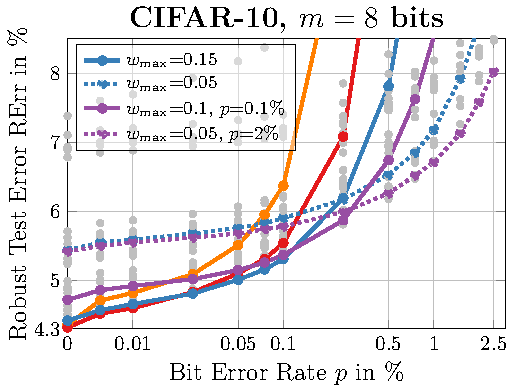
\includegraphics[height=3.075cm]{c10_summary_8bit.pdf}
	\end{subfigure}
	\begin{subfigure}{0.24\textwidth}
		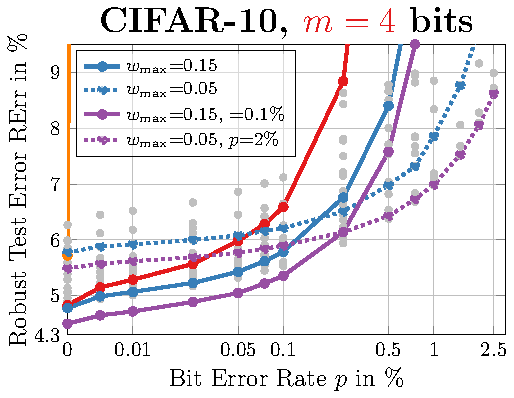
\includegraphics[height=3.1cm]{c10_summary_4bit.pdf}
	\end{subfigure}
	\begin{subfigure}{0.24\textwidth}
		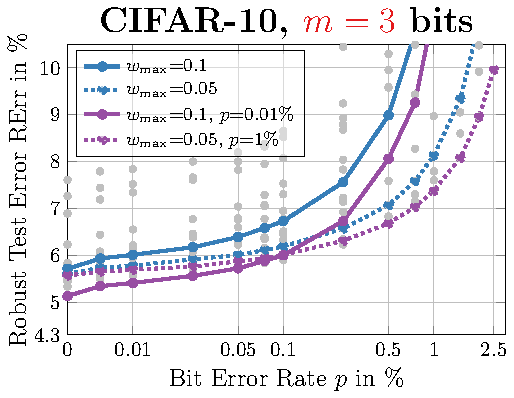
\includegraphics[height=3.1cm]{c10_summary_3bit.pdf}
	\end{subfigure}
	\begin{subfigure}{0.24\textwidth}
		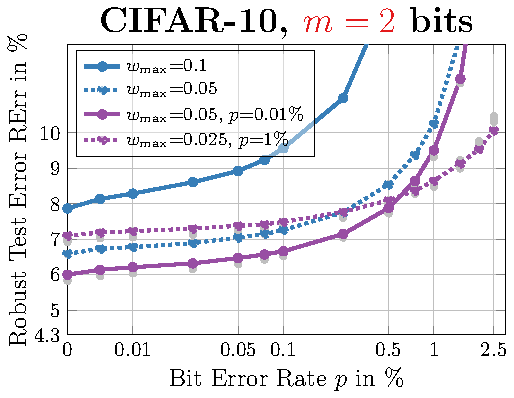
\includegraphics[height=3.1cm]{c10_summary_2bit.pdf}
	\end{subfigure}
	\\[2px]
	
	\begin{subfigure}{0.26\textwidth}
		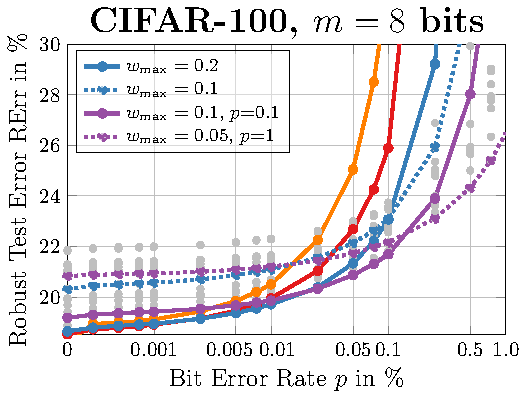
\includegraphics[height=3.1cm]{c100_summary_8bit.pdf}
	\end{subfigure}
	\begin{subfigure}{0.24\textwidth}
		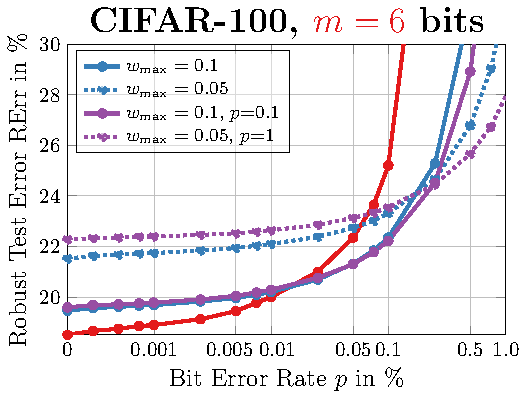
\includegraphics[height=3.1cm]{c100_summary_6bit.pdf}
	\end{subfigure}
	\begin{subfigure}{0.24\textwidth}
		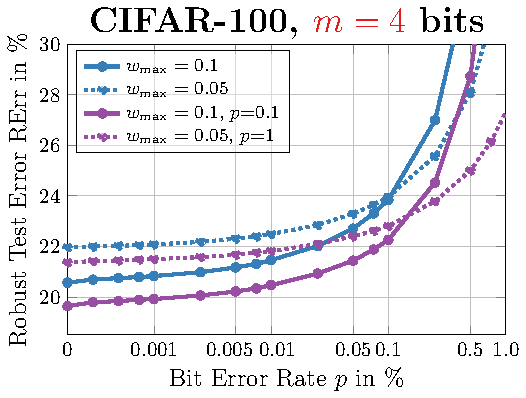
\includegraphics[height=3.1cm]{c100_summary_4bit.pdf} 
	\end{subfigure}
	\begin{subfigure}{0.24\textwidth}
		\hphantom{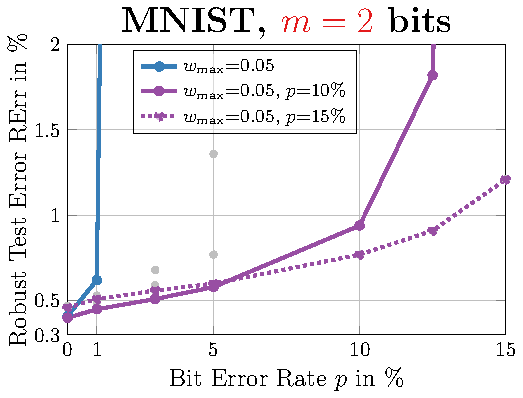
\includegraphics[height=3.45cm]{m_summary_2bit.pdf}}
	\end{subfigure}
	\\[2px]
	
	\begin{subfigure}{0.26\textwidth}
		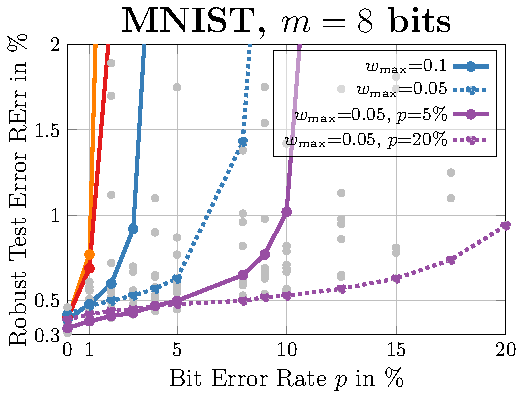
\includegraphics[height=3.1cm]{m_summary_8bit.pdf}
	\end{subfigure}
	\begin{subfigure}{0.24\textwidth}
		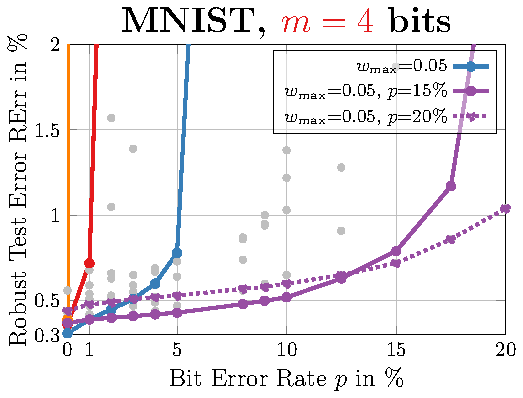
\includegraphics[height=3.1cm]{m_summary_4bit.pdf}
	\end{subfigure}
	\begin{subfigure}{0.24\textwidth}
		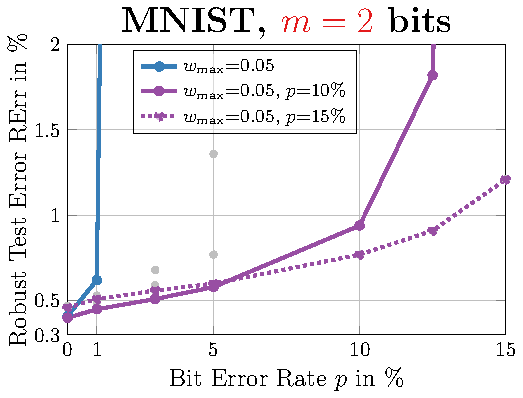
\includegraphics[height=3.1cm]{m_summary_2bit.pdf}
	\end{subfigure}
	\begin{subfigure}{0.24\textwidth}
		\hphantom{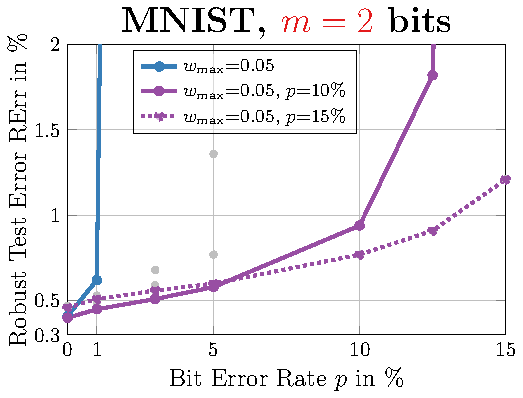
\includegraphics[height=3.45cm]{m_summary_2bit.pdf}}
	\end{subfigure}
	
	
	\hspace*{-0.1cm}
	\fbox{
	\begin{subfigure}{0.98\textwidth}
		\centering 
		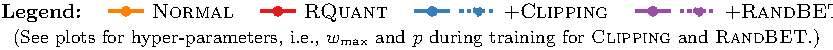
\includegraphics[width=0.8\textwidth]{c10_legend_supp}
	\end{subfigure}
	}
	\vspace*{-8px}
	\caption{\textbf{Summary Results on \CifarT, \CifarH and \MNIST.} Complementary to \figref{fig:summary}, we highlight individual \Clipping and \Random models. Note that \figref{fig:summary}, in contrast, presents the best, \ie, lowest \RTE, model for each bit error rate $p$ individually. Instead, individual models help to illustrate the involved trade-offs: \Clipping with small $\wmax$ or \Random with high bit error rate $p$ increases the clean \TE, thereby also increasing \RTE for very small bit error rates. However, \RTE against large bit error rates can be reduced significantly.}
	\label{fig:supp-summary}
\end{figure*}

In \tabref{tab:supp-randbet-baselines}, we follow the procedure of \appref{subsec:supp-errors-profiled} considering only persistent bit errors (\ie, where $p_{\text{1t0}}$ and $p_{\text{0t1}}$ are $1$). This is illustrated in \figref{fig:supp-errors} (right). Thus, the bit error rates deviate slightly from those reported in \tabref{tab:supp-randbet-generalization}, see the table in \appref{subsec:supp-errors-profiled} for details. Furthermore, We consider only one weight-to-SRAM mapping, \ie, without offset. \Pattern is trained and evaluated on the exact same bit error pattern, but potentially with different bit error rates $p$. Note that the bit errors for $p' < p$ are a subset of those for bit error rate $p$. Thus, it is surprising that, on both chips 1 and 2, \Pattern trained on higher bit error rates does not even generalize to lower bit error rates (\ie, higher voltage). This is problematic in practice as the DNN accelerator should not perform worse when increasing voltage.

\subsection{Guarantees from Prop. \ref{prop:bound}}
\label{subsec:experiments-stress}

Based on the bound derived in \secref{subsec:supp-bound}, we conduct experiments with $l = 1\text{Mio}$ random bit error patterns, such that $l \gg n$ where $n = \text{10k}$ is the number of test examples on \CifarT. Considering Prop. \ref{prop:bound}, this would guarantee a deviation in \RTE of at most $4.1\%$ with probability at least $99\%$. As shown in \tabref{tab:supp-stress}, the obtained \RTE with $1\text{Mio}$ random bit error patterns deviates insignificantly from the results in the main paper. Only standard deviation of \RTE increases slightly. These results emphasize that the results for \Clipping and \Random from the main paper generalize well.

\subsection{Other Architectures}
\label{subsec:supp-experiments-architectures}

\tabref{tab:supp-randbet-resnet} shows results on \CifarT using ResNet-20 and ResNet-50. We note that, in both cases, we use group normalization (GN) instead of batch normalization (BN) as outlined in \secref{subsec:supp-experiments-bn}. ResNet-50, in particular, suffers from using GN due to the significant depth: the clean \TE reduces from $3.67\%$ to $6.81\%$ in \tabref{tab:supp-accuracy}. Nevertheless, \Clipping and \Random remain effective against random bit errors, even for higher bit error rates of $p = 1.5\%$. This is striking as ResNet-50 consists of roughly $23.5\text{Mio}$ weights, compared to $5.5\text{Mio}$ of the used SimpleNet in the main paper.

\subsection{Summary Results}
\label{subsec:supp-experiments-summary}

\figref{fig:supp-summary} summarizes our results: In contrast to \figref{fig:summary}, we consider individual \Clipping and \Random models instead of focusing on the best results per bit error rate $p$. Additionally, we show our complete results for lower precisions, \ie, $m = 4,3,2$ on \CifarT and \MNIST. Note that these results, in tabular form, are included in \tabref{tab:supp-summary-cifar10} to \ref{tab:supp-summary-mnist}. Moderate \Clipping, \eg, using $\wmax = 0.15$ on \CifarT (in {\color{colorbrewer1}red}), has negligible impact on clean \TE (\ie, $p = 0$ on the x-axis) while improving robustness beyond $p = 0.1\%$ bit error rate. Generally, however, higher robustness is obtained at the cost of increased clean \TE, \eg, for $\wmax = 0.05$ (in {\color{colorbrewer2}blue}). Here, it is important to note that in low-voltage operation, only \RTE matters -- clean \TE is only relevant for voltages higher than \Vmin. \Random further improves robustness for high bit error rates, while continuing to increase clean \TE slightly. For example, \Random with $\wmax = 0.05$ and trained with $p = 2\%$ bit errors increases clean \TE to $5.42\%$ but is also able to keep \RTE below $7\%$ up to $p = 1\%$ bit error rate (in {\color{colorbrewer5}orange}). Reducing precision generally increases \TE and \RTE, especially for $m = 2$ bit. Here, our simple fixed-point quantization scheme is clearly limited compared to state-of-the-art. Nevertheless, even for $m = 2$ bits, \Random ({\color{colorbrewer4}violet} or {\color{colorbrewer5}orange}) is able to keep \RTE low until roughly $p = 0.1\%$ bit error rate. Note that for $m = 2$, more aggressive clipping generally helps during training and, thus, also reduces clean \TE (\cf $\wmax = 0.1$ and $\wmax = 0.05$ in {\color{colorbrewer1}red} and {\color{colorbrewer2}blue}).

Similar trade-offs can be observed on \CifarH and \MNIST. On \CifarH, we see that task difficulty also reduces the bit error rate that is tolerable without significant increase it \RTE. Here, $p = 0.1\%$ increases \RTE by more than $3\%$, even with \Random (and weight clipping). Furthermore, \CifarH demonstrates that \Clipping and \Random are applicable to significantly larger architectures such as Wide ResNets without problems. On \MNIST, in contrast, bit error rates of up to $p = 20\%$ are easily possible. At such bit error rates, the benefit of \Random is extremely significant as even \Clipping[$0.025$] exhibits very high \RTE of $32.68\%$ at $p = 20\%$, \cf \tabref{tab:supp-summary-mnist}.

\clearpage
\begin{table*}
	\centering
	\small
	\caption{\textbf{Overall Robustness Results on \CifarT.} Tabular results corresponding to \figref{fig:summary} and \ref{fig:supp-summary} for $m = 8$ and $m = 4$ bits. We show \RTE for \Normal, \Clipping and \Random with various $\wmax$ and $p$ across a subset of test bit error rates.}
	\label{tab:supp-summary-cifar10}
	\vspace*{-0.2cm}
	\begin{tabular}{| c | l | c | c | c | c | c | c | c | c | c |}
		\hline
		\multicolumn{11}{|c|}{\bfseries \CifarT: summary results for $\mathbf{m = 8}$ and  {\color{red}$\mathbf{m = 4}$} bit}\\
		\hline
		& Model & \multirow{2}{*}{\begin{tabular}{c}\TE\\in \%\end{tabular}} & \multicolumn{8}{c|}{\RTE in \%, $p$ in \% p=0.01}\\
		\cline{4-11}
		&&& $0.01$ & $0.05$ & $0.1$ & $0.5$ & $1$ & $1.5$ & $2$ & $2.5$\\
		\hline
		\hline
		\multirow{30}{*}{\rotatebox{90}{$m = 8$ bit}} & \Normal & 4.36 & 4.82 & 5.51 & 6.37 & 24.76 & 72.65 & 87.40 & 89.76 & 90.15\\
		& \Quant & 4.32 & 4.60 & 5.10 & 5.54 & 11.28 & 32.05 & 68.65 & 85.28 & 89.01\\
		& \Clipping[$0.25$] & 4.58 & 4.84 & 5.29 & 5.71 & 10.52 & 27.95 & 62.46 & 82.61 & 88.08\\
		& \Clipping[$0.2$] & 4.63 & 4.91 & 5.28 & 5.62 & 8.27 & 18.00 & 53.74 & 82.02 & 88.27\\
		& \Clipping[$0.15$] & 4.42 & 4.66 & 5.01 & 5.31 & 7.81 & 13.08 & 23.85 & 42.12 & 61.20\\
		& \Clipping[$0.1$] & 4.82 & 5.04 & 5.33 & 5.58 & 6.95 & 8.93 & 12.22 & 17.80 & 27.02\\
		& \Clipping[$0.05$] & 5.44 & 5.59 & 5.76 & 5.90 & 6.53 & 7.18 & 7.92 & 8.70 & 9.56\\
		& \Clipping[$0.025$] & 7.10 & 7.20 & 7.32 & 7.40 & 7.82 & 8.18 & 8.43 & 8.74 & --\\
		\cline{2-11}
		& \Random[$1$] $p{=}0.01$ & 4.56 & 4.93 & 5.50 & 6.06 & 14.14 & 66.07 & 86.86 & 89.80 & 90.35\\
		& \Random[$1$] $p{=}0.1$ & 4.50 & 4.80 & 5.27 & 5.72 & 10.33 & 41.10 & 75.90 & 86.52 & 89.03\\
		& \Random[$1$] $p{=}1$ & 7.38 & 7.69 & 8.17 & 8.58 & 11.10 & 14.90 & 21.08 & 41.11 & 71.09\\
		& \Random[$0.2$] $p{=}0.01$ & 4.44 & 4.67 & 5.09 & 5.48 & 8.64 & 17.97 & 41.53 & 68.95 & 82.48\\
		& \Random[$0.2$] $p{=}0.1$ & 4.51 & 4.73 & 5.07 & 5.39 & 7.99 & 19.21 & 54.94 & 80.12 & 86.55\\
		& \Random[$0.2$] $p{=}1$ & 5.46 & 5.68 & 5.97 & 6.20 & 7.63 & 9.47 & 12.38 & 21.47 & 50.86\\
		& \Random[$0.15$] $p{=}0.01$ & 4.64 & 4.87 & 5.17 & 5.45 & 7.54 & 15.83 & 54.07 & 81.41 & 86.75\\
		& \Random[$0.15$] $p{=}0.1$ & 4.86 & 5.07 & 5.36 & 5.64 & 7.74 & 12.33 & 22.38 & 40.09 & 60.78\\
		& \Random[$0.15$] $p{=}1$ & 5.27 & 5.44 & 5.68 & 5.88 & 7.11 & 8.63 & 11.13 & 27.74 & 64.97\\
		& \Random[$0.1$] $p{=}0.01$ & 4.99 & 5.15 & 5.39 & 5.62 & 6.93 & 9.01 & 12.83 & 22.81 & 41.04\\
		& \Random[$0.1$] $p{=}0.1$ & 4.72 & 4.92 & 5.15 & 5.37 & 6.74 & 8.53 & 11.40 & 15.97 & 23.59\\
		& \Random[$0.1$] $p{=}1$ & 4.90 & 5.05 & 5.26 & 5.43 & 6.36 & 7.41 & 8.65 & 12.25 & 27.21\\
		& \Random[$0.1$] $p{=}1.5$ & 5.53 & 5.67 & 5.87 & 6.03 & 6.84 & 7.76 & 8.80 & 10.03 & 11.68\\
		& \Random[$0.1$] $p{=}2$ & 5.71 & 5.87 & 6.07 & 6.22 & 7.00 & 7.83 & 8.69 & 9.70 & 10.91\\
		& \Random[$0.05$] $p{=}0.1$ & 5.32 & 5.41 & 5.59 & 5.72 & 6.34 & 6.96 & 7.62 & 8.28 & 9.13\\
		& \Random[$0.05$] $p{=}1$ & 5.24 & 5.36 & 5.50 & 5.60 & 6.18 & 6.73 & 7.26 & 7.88 & 8.49\\
		& \Random[$0.05$] $p{=}1.5$ & 5.62 & 5.71 & 5.84 & 5.95 & 6.50 & 7.02 & 7.52 & 7.97 & 8.51\\
		& \Random[$0.05$] $p{=}2$ & 5.42 & 5.55 & 5.68 & 5.78 & 6.26 & 6.71 & 7.13 & 7.58 & 8.02\\
		& \Random[$0.025$] $p{=}1$ & 6.78 & 6.88 & 7.00 & 7.08 & 7.46 & 7.75 & 8.02 & 8.24 & 8.47\\
		& \Random[$0.025$] $p{=}1.5$ & 6.89 & 6.99 & 7.11 & 7.19 & 7.58 & 7.94 & 8.26 & 8.52 & 8.77\\
		& \Random[$0.025$] $p{=}2$ & 6.93 & 7.02 & 7.12 & 7.20 & 7.57 & 7.87 & 8.11 & 8.33 & 8.58\\
		& \Random[$0.025$] $p{=}2.5$ & 6.91 & 6.99 & 7.08 & 7.14 & 7.50 & 7.83 & 8.10 & 8.36 & 8.63\\
		\hline
		\hline
		\multirow{19}{*}{\rotatebox{90}{$m = 4$ bit}} & \Quant & 4.83 & 5.29 & 5.98 & 6.59 & 15.72 & 50.45 & 79.86 & 87.17 & 89.47\\
		& \Clipping[$0.25$] & 4.78 & 5.16 & 5.75 & 6.26 & 12.08 & 30.62 & 60.52 & 80.07 & 87.01\\
		& \Clipping[$0.2$] & 4.90 & 5.20 & 5.65 & 6.04 & 9.67 & 27.24 & 63.96 & 82.63 & 87.21\\
		& \Clipping[$0.15$] & 4.78 & 5.07 & 5.43 & 5.79 & 8.40 & 14.61 & 28.53 & 50.83 & 70.32\\
		& \Clipping[$0.1$] & 5.29 & 5.49 & 5.75 & 5.99 & 7.71 & 10.62 & 15.79 & 24.97 & 37.94\\
		& \Clipping[$0.05$] & 5.78 & 5.92 & 6.08 & 6.21 & 6.98 & 7.86 & 8.77 & 9.76 & 11.04\\
		\cline{2-11}
		& \Random[$0.2$] $p{=}0.01$ & 5.14 & 5.42 & 5.85 & 6.23 & 10.44 & 23.84 & 49.25 & 73.35 & 83.16\\
		& \Random[$0.2$] $p{=}0.1$ & 4.77 & 5.01 & 5.41 & 5.76 & 8.66 & 16.06 & 32.40 & 56.69 & 75.21\\
		& \Random[$0.2$] $p{=}1$ & 6.27 & 6.52 & 6.86 & 7.12 & 8.78 & 11.33 & 15.17 & 21.43 & 32.19\\
		& \Random[$0.15$] $p{=}0.01$ & 4.88 & 5.13 & 5.54 & 5.92 & 8.51 & 14.21 & 26.26 & 46.02 & 66.13\\
		& \Random[$0.15$] $p{=}0.1$ & 4.50 & 4.72 & 5.05 & 5.36 & 7.58 & 14.12 & 43.00 & 76.28 & 85.54\\
		& \Random[$0.15$] $p{=}1$ & 5.99 & 6.18 & 6.45 & 6.65 & 8.00 & 9.74 & 12.50 & 16.73 & 24.09\\
		& \Random[$0.1$] $p{=}0.01$ & 5.07 & 5.29 & 5.58 & 5.83 & 7.54 & 10.46 & 15.34 & 24.63 & 39.76\\
		& \Random[$0.1$] $p{=}0.1$ & 4.82 & 5.04 & 5.32 & 5.53 & 6.82 & 8.85 & 12.48 & 21.36 & 40.03\\
		& \Random[$0.1$] $p{=}1$ & 5.39 & 5.55 & 5.77 & 5.96 & 7.04 & 8.34 & 9.77 & 11.85 & 14.91\\
		& \Random[$0.05$] $p{=}0.1$ & 5.14 & 5.26 & 5.46 & 5.61 & 6.38 & 7.19 & 8.06 & 9.16 & 10.46\\
		& \Random[$0.05$] $p{=}1$ & 5.60 & 5.71 & 5.85 & 5.97 & 6.54 & 7.10 & 7.68 & 8.28 & 8.99\\
		& \Random[$0.05$] $p{=}1.5$ & 5.51 & 5.64 & 5.77 & 5.87 & 6.38 & 6.98 & 7.51 & 8.10 & 8.72\\
		& \Random[$0.05$] $p{=}2$ & 5.49 & 5.62 & 5.77 & 5.90 & 6.43 & 6.99 & 7.53 & 8.06 & 8.62\\
		\hline
	\end{tabular}
	\vspace*{-0.2cm}
\end{table*}
\begin{table*}
	\centering
	\small
	\caption{\textbf{Overall Robustness Results on \CifarT.} \textbf{Overall Robustness Results on \CifarT.} Continued from \tabref{tab:supp-summary-cifar10}; tabular results corresponding to \figref{fig:summary} and \ref{fig:supp-summary} for $m = 3$ and $m = 2$ bits. We show \RTE for \Normal, \Clipping and \Random with various $\wmax$ and $p$ across a subset of test bit error rates.}
	\vspace*{-0.2cm}
	\begin{tabular}{| c | l | c | c | c | c | c | c | c | c | c |}
		\hline
		\multicolumn{11}{|c|}{\bfseries \CifarT: summary results for {\color{red}$\mathbf{m = 3}$} and {\color{red}$\mathbf{m = 2}$} bit}\\
		\hline
		& Model & \multirow{2}{*}{\begin{tabular}{c}\TE\\in \%\end{tabular}} & \multicolumn{8}{c|}{\RTE in \%, $p$ in \% p=0.01}\\
		\cline{4-11}
		&&& $0.01$ & $0.05$ & $0.1$ & $0.5$ & $1$ & $1.5$ & $2$ & $2.5$\\
		\hline
		\hline
		\multirow{20}{*}{\rotatebox{90}{$m = 3$ bit}} & \Quant & 79.59 & 83.95 & 88.57 & 91.07 & 96.15 & 97.81 & 98.20 & 98.60 & 99.07\\
		& \Clipping[$0.25$] & 6.89 & 7.34 & 8.00 & 8.65 & 14.46 & 28.70 & 53.64 & 75.51 & 85.13\\
		& \Clipping[$0.2$] & 5.82 & 6.21 & 6.79 & 7.30 & 11.90 & 23.31 & 43.00 & 65.68 & 78.79\\
		& \Clipping[$0.15$] & 5.84 & 6.16 & 6.60 & 6.95 & 9.95 & 15.92 & 27.84 & 47.54 & 67.08\\
		& \Clipping[$0.1$] & 5.71 & 6.01 & 6.39 & 6.73 & 8.99 & 13.06 & 20.88 & 35.13 & 51.76\\
		& \Clipping[$0.05$] & 5.61 & 5.78 & 6.01 & 6.19 & 7.07 & 8.13 & 9.34 & 10.95 & 13.16\\
		\cline{2-11}
		& \Random[$0.2$] $p{=}0.01$ & 5.72 & 6.14 & 6.77 & 7.30 & 12.84 & 26.46 & 50.52 & 72.46 & 83.09\\
		& \Random[$0.2$] $p{=}0.1$ & 6.23 & 6.55 & 7.04 & 7.53 & 11.38 & 21.36 & 41.93 & 65.54 & 79.94\\
		& \Random[$0.2$] $p{=}1$ & 7.61 & 7.84 & 8.20 & 8.52 & 10.30 & 12.82 & 16.65 & 21.81 & 29.64\\
		& \Random[$0.15$] $p{=}0.01$ & 5.61 & 5.94 & 6.40 & 6.77 & 9.59 & 15.72 & 28.06 & 46.88 & 64.39\\
		& \Random[$0.15$] $p{=}0.1$ & 5.33 & 5.56 & 5.99 & 6.33 & 9.01 & 14.06 & 23.44 & 40.36 & 59.92\\
		& \Random[$0.15$] $p{=}1$ & 7.26 & 7.52 & 7.82 & 8.07 & 9.58 & 11.47 & 13.87 & 17.58 & 23.01\\
		& \Random[$0.1$] $p{=}0.01$ & 5.13 & 5.41 & 5.72 & 6.00 & 8.06 & 11.25 & 17.22 & 26.96 & 42.72\\
		& \Random[$0.1$] $p{=}0.1$ & 5.69 & 5.96 & 6.26 & 6.51 & 8.04 & 10.81 & 15.51 & 23.88 & 37.52\\
		& \Random[$0.1$] $p{=}1$ & 5.76 & 5.95 & 6.22 & 6.44 & 7.59 & 8.97 & 10.76 & 13.21 & 16.95\\
		& \Random[$0.05$] $p{=}0.01$ & 5.50 & 5.62 & 5.83 & 5.99 & 6.83 & 7.79 & 9.05 & 10.48 & 12.32\\
		& \Random[$0.05$] $p{=}0.1$ & 5.44 & 5.58 & 5.76 & 5.90 & 6.72 & 7.60 & 8.60 & 9.92 & 11.70\\
		& \Random[$0.05$] $p{=}1$ & 5.57 & 5.69 & 5.87 & 6.01 & 6.68 & 7.38 & 8.08 & 8.96 & 9.96\\
		\hline
		\hline
		\multirow{11}{*}{\rotatebox{90}{$m = 2$ bit}} & \Quant & 88.68 & 89.53 & 91.62 & 93.23 & 97.74 & 98.40 & 97.85 & 99.20 & 98.74\\
		& \Clipping[$0.25$] & 90.14 & 90.54 & 91.13 & 91.82 & 95.96 & 96.90 & 97.21 & 96.66 & 97.12\\
		& \Clipping[$0.2$] & 82.00 & 84.86 & 90.79 & 94.17 & 97.25 & 96.69 & 97.16 & 97.73 & 97.01\\
		& \Clipping[$0.15$] & 14.62 & 15.29 & 16.30 & 17.16 & 22.88 & 33.18 & 50.86 & 71.17 & 84.30\\
		& \Clipping[$0.1$] & 7.87 & 8.29 & 8.93 & 9.57 & 13.95 & 23.65 & 42.43 & 64.65 & 80.89\\
		& \Clipping[$0.05$] & 6.59 & 6.78 & 7.05 & 7.26 & 8.55 & 10.26 & 12.73 & 15.99 & 20.51\\
		& \Clipping[$0.025$] & 6.94 & 7.06 & 7.23 & 7.34 & 7.96 & 8.57 & 9.16 & 9.77 & 10.47\\
		& \Random[$0.05$] $p{=}0.01$ & 6.00 & 6.21 & 6.47 & 6.66 & 7.88 & 9.51 & 11.53 & 14.99 & 19.60\\
		& \Random[$0.05$] $p{=}0.1$ & 5.83 & 6.04 & 6.30 & 6.52 & 7.73 & 9.32 & 11.41 & 14.49 & 19.77\\
		& \Random[$0.025$] $p{=}0.01$ & 6.93 & 7.07 & 7.24 & 7.37 & 8.05 & 8.65 & 9.23 & 9.72 & 10.43\\
		& \Random[$0.025$] $p{=}0.1$ & 7.02 & 7.13 & 7.31 & 7.41 & 7.98 & 8.48 & 9.00 & 9.65 & 10.32\\
		& \Random[$0.025$] $p{=}1$ & 7.10 & 7.23 & 7.38 & 7.49 & 8.10 & 8.65 & 9.14 & 9.54 & 10.07\\
		\hline
	\end{tabular}
\end{table*}
\begin{table*}
	\centering
	\small
	\caption{\textbf{Overall Robustness Results on \CifarH.} Tabular results corresponding to \figref{fig:summary} and \ref{fig:supp-summary} for $m = 8$. We show \RTE for \Normal, \Clipping and \Random with various $\wmax$ and $p$ across a subset of test bit error rates.}
	\label{tab:supp-summary-cifar100}
	\vspace*{-0.2cm}
	\begin{tabular}{|l | c | c | c | c | c | c | c |}
		\hline
		\multicolumn{8}{|c|}{\bfseries \CifarH: summary results for $\mathbf{m = 8}$ bit}\\
		\hline
		Model & \multirow{2}{*}{\begin{tabular}{c}\TE\\in \%\end{tabular}} & \multicolumn{6}{c|}{\RTE in \%, $p$ in \% p=0.01}\\
		\cline{3-8}
		&& $0.005$ & $0.01$ & $0.05$ & $0.1$ & $0.5$ & $1$\\
		\hline
		\hline
		\Normal & 18.21 & 19.84 {\color{gray}\scriptsize ${\pm}$0.16} & 20.50 {\color{gray}\scriptsize ${\pm}$0.25} & 25.05 {\color{gray}\scriptsize ${\pm}$0.94} & 32.39 {\color{gray}\scriptsize ${\pm}$1.89} & 97.49 {\color{gray}\scriptsize ${\pm}$0.95} & 99.10 {\color{gray}\scriptsize ${\pm}$0.19}\\
		\Quant & 18.53 & 19.46 {\color{gray}\scriptsize ${\pm}$0.13} & 19.95 {\color{gray}\scriptsize ${\pm}$0.16} & 22.68 {\color{gray}\scriptsize ${\pm}$0.63} & 25.90 {\color{gray}\scriptsize ${\pm}$1.01} & 87.24 {\color{gray}\scriptsize ${\pm}$3.99} & 98.77 {\color{gray}\scriptsize ${\pm}$0.31}\\
		\Clipping[$0.25$] & 18.88 & 19.76 {\color{gray}\scriptsize ${\pm}$0.1} & 20.11 {\color{gray}\scriptsize ${\pm}$0.11} & 21.89 {\color{gray}\scriptsize ${\pm}$0.18} & 23.74 {\color{gray}\scriptsize ${\pm}$0.35} & 62.25 {\color{gray}\scriptsize ${\pm}$4.51} & 96.62 {\color{gray}\scriptsize ${\pm}$1.22}\\
		\Clipping[$0.2$] & 18.64 & 19.36 {\color{gray}\scriptsize ${\pm}$0.09} & 19.71 {\color{gray}\scriptsize ${\pm}$0.1} & 21.33 {\color{gray}\scriptsize ${\pm}$0.23} & 23.07 {\color{gray}\scriptsize ${\pm}$0.38} & 49.79 {\color{gray}\scriptsize ${\pm}$4.21} & 94.02 {\color{gray}\scriptsize ${\pm}$2.38}\\
		\Clipping[$0.15$] & 19.41 & 20.00 {\color{gray}\scriptsize ${\pm}$0.08} & 20.24 {\color{gray}\scriptsize ${\pm}$0.09} & 21.68 {\color{gray}\scriptsize ${\pm}$0.17} & 23.02 {\color{gray}\scriptsize ${\pm}$0.3} & 37.85 {\color{gray}\scriptsize ${\pm}$2.03} & 79.45 {\color{gray}\scriptsize ${\pm}$5.08}\\
		\Clipping[$0.1$] & 20.31 & 20.86 {\color{gray}\scriptsize ${\pm}$0.07} & 21.09 {\color{gray}\scriptsize ${\pm}$0.09} & 22.14 {\color{gray}\scriptsize ${\pm}$0.17} & 23.10 {\color{gray}\scriptsize ${\pm}$0.21} & 31.78 {\color{gray}\scriptsize ${\pm}$1.15} & 51.71 {\color{gray}\scriptsize ${\pm}$3.47}\\
		\Clipping[$0.05$] & 21.82 & 22.16 {\color{gray}\scriptsize ${\pm}$0.05} & 22.29 {\color{gray}\scriptsize ${\pm}$0.06} & 22.94 {\color{gray}\scriptsize ${\pm}$0.13} & 23.46 {\color{gray}\scriptsize ${\pm}$0.18} & 26.86 {\color{gray}\scriptsize ${\pm}$0.46} & 31.47 {\color{gray}\scriptsize ${\pm}$0.79}\\
		\hline
		\Random[$0.1$] $p{=}0.01$ & 19.68 & 20.21 {\color{gray}\scriptsize ${\pm}$0.08} & 20.46 {\color{gray}\scriptsize ${\pm}$0.09} & 21.52 {\color{gray}\scriptsize ${\pm}$0.17} & 22.56 {\color{gray}\scriptsize ${\pm}$0.25} & 30.59 {\color{gray}\scriptsize ${\pm}$0.82} & 48.93 {\color{gray}\scriptsize ${\pm}$3.31}\\
		\Random[$0.1$] $p{=}0.05$ & 19.94 & 20.47 {\color{gray}\scriptsize ${\pm}$0.06} & 20.69 {\color{gray}\scriptsize ${\pm}$0.08} & 21.72 {\color{gray}\scriptsize ${\pm}$0.16} & 22.60 {\color{gray}\scriptsize ${\pm}$0.23} & 29.93 {\color{gray}\scriptsize ${\pm}$0.86} & 46.76 {\color{gray}\scriptsize ${\pm}$3.46}\\
		\Random[$0.1$] $p{=}0.1$ & 19.18 & 19.67 {\color{gray}\scriptsize ${\pm}$0.06} & 19.86 {\color{gray}\scriptsize ${\pm}$0.07} & 20.87 {\color{gray}\scriptsize ${\pm}$0.12} & 21.69 {\color{gray}\scriptsize ${\pm}$0.21} & 28.03 {\color{gray}\scriptsize ${\pm}$0.74} & 41.29 {\color{gray}\scriptsize ${\pm}$2.81}\\
		\Random[$0.1$] $p{=}0.5$ & 19.90 & 20.24 {\color{gray}\scriptsize ${\pm}$0.05} & 20.41 {\color{gray}\scriptsize ${\pm}$0.07} & 21.17 {\color{gray}\scriptsize ${\pm}$0.13} & 21.83 {\color{gray}\scriptsize ${\pm}$0.17} & 25.66 {\color{gray}\scriptsize ${\pm}$0.48} & 31.55 {\color{gray}\scriptsize ${\pm}$0.95}\\
		\Random[$0.1$] $p{=}1$ & 21.08 & 21.43 {\color{gray}\scriptsize ${\pm}$0.05} & 21.59 {\color{gray}\scriptsize ${\pm}$0.07} & 22.24 {\color{gray}\scriptsize ${\pm}$0.13} & 22.76 {\color{gray}\scriptsize ${\pm}$0.15} & 25.73 {\color{gray}\scriptsize ${\pm}$0.33} & 29.31 {\color{gray}\scriptsize ${\pm}$0.56}\\
		\Random[$0.05$] $p{=}0.01$ & 21.86 & 22.17 {\color{gray}\scriptsize ${\pm}$0.06} & 22.31 {\color{gray}\scriptsize ${\pm}$0.05} & 23.00 {\color{gray}\scriptsize ${\pm}$0.14} & 23.57 {\color{gray}\scriptsize ${\pm}$0.2} & 26.84 {\color{gray}\scriptsize ${\pm}$0.46} & 31.33 {\color{gray}\scriptsize ${\pm}$0.79}\\
		\Random[$0.05$] $p{=}0.05$ & 20.97 & 21.30 {\color{gray}\scriptsize ${\pm}$0.05} & 21.44 {\color{gray}\scriptsize ${\pm}$0.07} & 22.12 {\color{gray}\scriptsize ${\pm}$0.14} & 22.72 {\color{gray}\scriptsize ${\pm}$0.16} & 25.95 {\color{gray}\scriptsize ${\pm}$0.34} & 30.14 {\color{gray}\scriptsize ${\pm}$0.59}\\
		\Random[$0.05$] $p{=}0.1$ & 21.22 & 21.53 {\color{gray}\scriptsize ${\pm}$0.05} & 21.66 {\color{gray}\scriptsize ${\pm}$0.05} & 22.29 {\color{gray}\scriptsize ${\pm}$0.12} & 22.81 {\color{gray}\scriptsize ${\pm}$0.17} & 25.88 {\color{gray}\scriptsize ${\pm}$0.39} & 29.93 {\color{gray}\scriptsize ${\pm}$0.83}\\
		\Random[$0.05$] $p{=}0.5$ & 21.29 & 21.55 {\color{gray}\scriptsize ${\pm}$0.04} & 21.65 {\color{gray}\scriptsize ${\pm}$0.06} & 22.13 {\color{gray}\scriptsize ${\pm}$0.12} & 22.60 {\color{gray}\scriptsize ${\pm}$0.15} & 25.01 {\color{gray}\scriptsize ${\pm}$0.3} & 27.70 {\color{gray}\scriptsize ${\pm}$0.5}\\
		\Random[$0.05$] $p{=}1$ & 20.83 & 21.08 {\color{gray}\scriptsize ${\pm}$0.04} & 21.20 {\color{gray}\scriptsize ${\pm}$0.06} & 21.73 {\color{gray}\scriptsize ${\pm}$0.13} & 22.16 {\color{gray}\scriptsize ${\pm}$0.13} & 24.33 {\color{gray}\scriptsize ${\pm}$0.24} & 26.49 {\color{gray}\scriptsize ${\pm}$0.38}\\
		\hline
	\end{tabular}
\end{table*}
\begin{table*}
	\centering
	\small
	\caption{\textbf{Overall Robustness Results on \MNIST.} Tabular results corresponding to \figref{fig:summary} and \ref{fig:supp-summary} for $m = 8, 4, 2$ bits. We show \RTE for \Normal, \Clipping and \Random with various $\wmax$ and $p$ across a subset of test bit error rates.}
	\label{tab:supp-summary-mnist}
	\vspace*{-0.2cm}
	\begin{tabular}{| c | l | c | c | c | c | c | c | c | c |}
		\hline
		\multicolumn{10}{|c|}{\bfseries MNIST: summary results for $\mathbf{m = 8, 4, 3}$ bit}\\
		\hline
		& Model & \multirow{2}{*}{\begin{tabular}{c}\TE\\in \%\end{tabular}} & \multicolumn{7}{c|}{\RTE in \%, $p$ in \% p=0.01}\\
		\cline{3-10}
		&&& $1$ & $5$ & $10$ & $12.5$ & $15$ & $17.5$ & $20$\\
		\hline
		\hline
		\multirow{11}{*}{$m = 8$ bit} & \Normal & 0.39 & 0.77 & 86.37 & 89.92 & 89.82 & 89.81 & 90.09 & 90.03\\
		& \Quant & 0.40 & 0.69 & 85.96 & 90.20 & 89.86 & 90.10 & 89.72 & 89.83\\
		& \Clipping[$0.1$] & 0.39 & 0.48 & 18.21 & 88.93 & 90.35 & 90.06 & 90.56 & 90.18\\
		& \Clipping[$0.05$] & 0.42 & 0.47 & 0.63 & 8.67 & 51.38 & 80.64 & 87.79 & 89.57\\
		& \Clipping[$0.025$] & 0.43 & 0.47 & 0.56 & 0.71 & 0.95 & 1.81 & 7.22 & 32.68\\
		\cline{2-10}
		& \Random[$0.1$] $p{=}1$ & 0.36 & 0.44 & 3.41 & 86.29 & 89.05 & 89.85 & 90.10 & 89.93\\
		& \Random[$0.05$] $p{=}1$ & 0.34 & 0.39 & 0.59 & 8.92 & 51.32 & 79.35 & 87.63 & 89.15\\
		& \Random[$0.05$] $p{=}5$ & 0.34 & 0.38 & 0.50 & 1.02 & 5.12 & 41.31 & 79.19 & 87.88\\
		& \Random[$0.05$] $p{=}10$ & 0.40 & 0.43 & 0.51 & 0.67 & 0.86 & 1.74 & 9.77 & 47.58\\
		& \Random[$0.05$] $p{=}15$ & 0.39 & 0.40 & 0.45 & 0.56 & 0.64 & 0.78 & 1.10 & 2.72\\
		& \Random[$0.05$] $p{=}20$ & 0.39 & 0.42 & 0.48 & 0.53 & 0.57 & 0.63 & 0.74 & 0.94\\
		\hline
		\hline
		\multirow{14}{*}{$m = 4$ bit} & \Quant & 0.36 & 0.72 & 87.21 & 90.23 & 90.01 & 89.88 & 89.97 & 89.67\\
		& \Clipping[$0.1$] & 0.38 & 0.51 & 38.75 & 88.33 & 89.47 & 89.57 & 90.10 & 89.67\\
		& \Clipping[$0.05$] & 0.31 & 0.39 & 0.78 & 44.15 & 78.64 & 87.32 & 89.03 & 89.71\\
		& \Clipping[$0.025$] & 0.37 & 0.41 & 0.50 & 0.67 & 0.99 & 4.63 & 29.46 & 67.21\\
		\cline{2-10}
		& \Random[$0.1$] $p{=}1$ & 0.38 & 0.48 & 13.29 & 87.43 & 89.70 & 89.63 & 89.41 & 90.02\\
		& \Random[$0.1$] $p{=}5$ & 0.38 & 0.48 & 0.78 & 24.73 & 74.88 & 87.04 & 88.72 & 89.55\\
		& \Random[$0.1$] $p{=}10$ & 0.40 & 0.47 & 0.64 & 1.22 & 2.62 & 16.72 & 64.33 & 83.80\\
		& \Random[$0.1$] $p{=}15$ & 0.56 & 0.59 & 0.73 & 1.03 & 1.28 & 1.87 & 3.71 & 14.39\\
		& \Random[$0.1$] $p{=}20$ & 0.56 & 9.48 & 14.29 & 7.39 & 6.07 & 5.80 & 6.10 & 8.12\\
		& \Random[$0.05$] $p{=}1$ & 0.37 & 0.43 & 0.67 & 36.99 & 77.12 & 85.97 & 88.62 & 89.94\\
		& \Random[$0.05$] $p{=}5$ & 0.38 & 0.42 & 0.53 & 1.38 & 12.90 & 60.73 & 83.69 & 88.75\\
		& \Random[$0.05$] $p{=}10$ & 0.34 & 0.39 & 0.47 & 0.65 & 0.91 & 2.11 & 19.15 & 71.25\\
		& \Random[$0.05$] $p{=}15$ & 0.37 & 0.39 & 0.43 & 0.52 & 0.63 & 0.79 & 1.17 & 3.16\\
		& \Random[$0.05$] $p{=}20$ & 0.44 & 0.48 & 0.53 & 0.60 & 0.65 & 0.72 & 0.86 & 1.04\\
		\hline
		\hline
		\multirow{6}{*}{$m = 2$ bit} & \Clipping[$0.1$] & 0.47 & 3.82 & 89.19 & 89.92 & 90.22 & 90.14 & \multicolumn{2}{c}{\hphantom{c}}\\
		& \Clipping[$0.05$] & 0.41 & 0.62 & 77.19 & 89.47 & 90.40 & 90.06 & \multicolumn{2}{c}{\hphantom{c}}\\
		\cline{2-8}
		& \Random[$0.05$] $p{=}3$ & 0.47 & 0.53 & 1.36 & 82.71 & 88.66 & 90.28 & \multicolumn{2}{c}{\hphantom{c}}\\
		& \Random[$0.05$] $p{=}5$ & 0.40 & 0.49 & 0.77 & 25.72 & 78.71 & 88.22 & \multicolumn{2}{c}{\hphantom{c}}\\
		& \Random[$0.05$] $p{=}10$ & 0.40 & 0.45 & 0.58 & 0.94 & 1.82 & 15.70 & \multicolumn{2}{c}{\hphantom{c}}\\
		& \Random[$0.05$] $p{=}15$ & 0.46 & 0.51 & 0.60 & 0.77 & 0.91 & 1.21 & \multicolumn{2}{c}{\hphantom{c}}\\
		\cline{1-8}
	\end{tabular}
\end{table*}